\documentclass[11pt, titlepage]{article}
\author{Caleb Logemann}
\title{MATH 666: Finite Element Methods \\ Homework 2}
\date{October 23, 2018}
\usepackage[letterpaper, margin=2cm]{geometry}
\usepackage{MATH666}
\usepackage{booktabs}

\begin{document}
\maketitle

%\lstinputlisting[language=MATLAB]{H01_23.m}
\begin{enumerate}
  \item[\#1]
    Consider the 2D Poisson equation:
    \begin{align*}
      \mathbf{PDE}:& \quad -\nabla \cdot \nabla u = f(x, y) \quad \text{in} \quad \Omega = \br{-1,1} \times \br{-1,1} \\
      \mathbf{BC}:& \quad u + \nabla u \cdot \hat{\v{n}} = g \quad \text{on} \quad  \partial\Omega
    \end{align*}
    \begin{enumerate}
      \item[(a)]
        Recast this problem as a variational problem.
        Clearly state the test and trial function spaces.

        In order to recast this as a variational problem, I will multiply by a
        test function and integrate over $\Omega$.
        \begin{align*}
          \diintt{\Omega}{}{-\p{\nabla \cdot \nabla u} v}{\v{x}} &= \diintt{\Omega}{}{f v}{\v{x}}
          \intertext{Integrating by parts gives}
          \diintt{\Omega}{}{\nabla u \cdot \nabla v}{\v{x}} - \dintt{\partial\Omega}{}{\p{\nabla u \cdot \hat{\v{n}}} v}{s} &= \diintt{\Omega}{}{f v}{\v{x}}
          \intertext{Using the boundary condition we see that $\nabla u \cdot \hat{\v{n}} = g - u$ on $\partial \Omega$}
          \diintt{\Omega}{}{\nabla u \cdot \nabla v}{\v{x}} - \dintt{\partial\Omega}{}{\p{g - u} v}{s} &= \diintt{\Omega}{}{f v}{\v{x}} \\
          \diintt{\Omega}{}{\nabla u \cdot \nabla v}{\v{x}} + \dintt{\partial\Omega}{}{uv}{s} &= \diintt{\Omega}{}{f v}{\v{x}} + \dintt{\partial \Omega}{}{gv}{s} \\
        \end{align*}
        In order for this equation to be well defined $u$ and $v$ must be in
        the space $H^1(\Omega)$, that is they are square integrable on $\Omega$
        and the norm of their gradients are square integrable on $\Omega$.
        Note that being in $H^1(\Omega)$ implies $L^2(\partial \Omega)$, so the
        boundary integrals are also well defined.

        So the bilinear form of this variational problem is to find $u \in H^1(\Omega)$ such that
        \[
          B(u, v) = L(v)
        \]
        for all $v \in H^1(\Omega)$, where
        \[
          B(u,  v) = \diintt{\Omega}{}{\nabla u \cdot \nabla v}{\v{x}} + \dintt{\partial\Omega}{}{uv}{s}
        \]
        and
        \[
          L(v) = \diintt{\Omega}{}{f v}{\v{x}} + \dintt{\partial \Omega}{}{gv}{s}.
        \]

      \item[(b)]
        Show that the variational problem has a unique solution by showing that
        it meets all of the criteria of the Lax-Milgram Theorem.

        The four conditions of the Lax-Milgram Theorem are symmetry, continuity
        of $B$, V-ellipticity, and continuity of $L$, and are shown below.
        \begin{align*}
          B(u, v) &= B(v, u) \\
          \abs{B(u, v)} &\le \gamma \norm[V]{u} \norm[V]{v} \\
          B(v, v) &\ge \alpha \norm[V]{v}^2 \\
          \abs{L(v)} &\le \Gamma \norm[V]{v}
        \end{align*}

        I will show these four conditions in order.
        First, symmetry
        \begin{align*}
          B(u, v) &= \diintt{\Omega}{}{\nabla u \cdot \nabla v}{\v{x}} + \dintt{\partial\Omega}{}{uv}{s} \\
          &= \diintt{\Omega}{}{\nabla v \cdot \nabla u}{\v{x}} + \dintt{\partial\Omega}{}{vu}{s} \\
          &= B(v, u)
        \end{align*}
        Second, boundedness of $B$
        \begin{align*}
          \abs{B(u, v)} &= \abs{\diintt{\Omega}{}{\nabla u \cdot \nabla v}{\v{x}} + \dintt{\partial\Omega}{}{uv}{s}} \\
          &\le \abs{\diintt{\Omega}{}{\nabla u \cdot \nabla v}{\v{x}}} + \abs{\dintt{\partial\Omega}{}{uv}{s}}
          \intertext{Using Cauchy-Schwarz on both integrals gives}
          &\le \norm[L^2(\Omega)]{\norm{\nabla u}} \norm[L^2(\Omega)]{\norm{\nabla v}} + \norm[L^2(\partial\Omega)]{u}\norm[L^2(\partial\Omega)]{v}
          \intertext{Since $\partial\Omega \subset \Omega$, this implies that $\norm[L^2(\partial\Omega)]{u} \le \norm[L^2(\Omega)]{u}$, so}
          &\le \norm[L^2(\Omega)]{\norm{\nabla u}} \norm[L^2(\Omega)]{\norm{\nabla v}} + \norm[L^2(\Omega)]{u}\norm[L^2(\Omega)]{v}
          \intertext{Now since $\norm[H^1(\Omega)]{u}$ is greater than both $\norm[L^2(\Omega)]{\norm{\nabla u}}$ and $\norm[L^2(\Omega)]{u}$}
          \abs{B(u, v)} &\le 2\norm[H^1(\Omega)]{u} \norm[H^1(\Omega)]{v}
        \end{align*}
        Third I will show V-ellipticity of $B$.
        There are two possible cases $v = 0$ on $\partial \Omega$ or $v \neq 0$
        on $\partial \Omega$.
        If $v = 0$ on $\partial \Omega$, then
        \begin{align*}
          B(v, v) &= \diintt{\Omega}{}{\norm{\nabla v}^2}{\v{x}} + \dintt{\partial\Omega}{}{v^2}{s} \\
          &= \diintt{\Omega}{}{\norm{\nabla v}^2}{\v{x}} \\
          &= \frac{1}{2}\p{\diintt{\Omega}{}{\norm{\nabla v}^2}{\v{x}} + \diintt{\Omega}{}{\norm{\nabla v}^2}{\v{x}}} \\
          &= \frac{1}{2}\p{\norm[L^2(\Omega)]{\norm{\nabla v}}^2 + \norm[L^2(\Omega)]{\norm{\nabla v}}^2}
          \intertext{Poincare's Inequality states that there exists a constant
          $C > 0$ such that $C\norm[L^2(\Omega)]{v}^2 \le \norm[L^2(\Omega)]{\norm{\nabla v}}^2$, therefore}
          B(v, v) &\ge \frac{1}{2}\p{\norm[L^2(\Omega)]{\norm{\nabla v}}^2 + C\norm[L^2(\Omega)]{v}^2} \\
          &\ge \frac{1}{2}\min{1, C}\p{\norm[L^2(\Omega)]{\norm{\nabla v}}^2 + \norm[L^2(\Omega)]{v}^2} \\
          &= \frac{1}{2}\min{1, C} \norm[H^1(\Omega)]{v}
        \end{align*}
        If $v \neq 0$ on $\partial \Omega$, then we can make use of Friedrich's
        Inequality, which states that there exists constants $C_1 > 0$ and
        $C_2 > 0$ such that
        \[
          \diintt{\Omega}{}{v^2}{\v{x}} \le C_1\diintt{\Omega}{}{\norm{\nabla v}^2}{x} + C_2 \dintt{\partial\Omega}{}{v^2}{s}
        \]
        This is equivalent to
        \[
          \frac{1}{C}\diintt{\Omega}{}{v^2}{\v{x}} \le \diintt{\Omega}{}{\norm{\nabla v}^2}{x} + \dintt{\partial\Omega}{}{v^2}{s}
        \]
        where $C = \max{C_1, C_2}$.
        Now,
        \begin{align*}
          B(v, v) &= \diintt{\Omega}{}{\norm{\nabla v}^2}{\v{x}} + \dintt{\partial\Omega}{}{v^2}{s} \\
          &\ge \frac{1}{2}\diintt{\Omega}{}{\norm{\nabla v}^2}{\v{x}} + \frac{1}{2}\p{\diintt{\Omega}{}{\norm{\nabla v}^2}{\v{x}} + \dintt{\partial\Omega}{}{v^2}{s}}
          \intertext{Using Friedrich's Inequality}
          &\ge \frac{1}{2}\diintt{\Omega}{}{\norm{\nabla v}^2}{\v{x}} + \frac{1}{2C}\diintt{\Omega}{}{v^2}{\v{x}} \\
          &\ge \min{1, \frac{1}{C}}\p{\diintt{\Omega}{}{\norm{\nabla v}^2}{\v{x}} + \diintt{\Omega}{}{v^2}{\v{x}}} \\
          &= \min{1, \frac{1}{C}}\norm[H^1(\Omega)]{v} \\
        \end{align*}
        Therefore $B$ is V-elliptic.

        Lastly I will show that $L$ is bounded,
        \begin{align*}
          \abs{L(v)} &= \abs{\diintt{\Omega}{}{f v}{\v{x}} + \dintt{\partial \Omega}{}{gv}{s}} \\
          &\le \abs{\diintt{\Omega}{}{f v}{\v{x}}} + \abs{\dintt{\partial \Omega}{}{gv}{s}}
          \intertext{Using Cauchy-Schwarz on both integrals gives}
          &\le \norm[L^2(\Omega)]{f}\norm[L^2(\Omega)]{v} + \norm[L^2(\partial \Omega)]{g}\norm[L^2(\partial \Omega)]{v}
          \intertext{Now since $\norm[H^1(\Omega)]{v}$ is greater than both $\norm[L^2(\Omega)]{v}$ and $\norm[L^2(\partial\Omega)]{v}$}
          &\le \norm[L^2(\Omega)]{f}\norm[H^1(\Omega)]{v} + \norm[L^2(\partial \Omega)]{g}\norm[H^1(\Omega)]{v} \\
          &\le 2\max{\norm[L^2(\Omega)]{f}, \norm[L^2(\partial \Omega)]{g}}\norm[H^1(\Omega)]{v}
        \end{align*}
        This shows that the variational problem satisfies all of the criteria
        for the Lax-Milgram theorem, therefore it has a unique solution.

      \item[(c)]
        Develop a finite element method for this problem based on square elements.
        On each element, the solution on the four corners is interpolated with the
        following interpolant:
        \[
          s(x, y) = \alpha_1 + \alpha_2 x + \alpha_3 y + \alpha_4 x y.
        \]
        Write out the basis functions and explicitly write out the linear system
        that arises from your FEM(you can assume that the grid spacing in $x$
        and $y$ are the same and uniform).

        There will be a basis function for each node on the grid.
        Since we are implicitly enforcing the boundary conditions through the
        variational problem, all of the basis function can be the same.
        We don't need different basis functions for the boundary.
        Note that the basis functions corresponding with nodes on the boundary
        will have some support outside $\Omega$ which will be ignored in
        future integrals.
        I will let $M$ denote the number of points in one direction, so there
        will be $N = M^2$ total nodes on the grid.
        I will use a row-wise numbering of these nodes, that is the first row of
        nodes will be numbered $1 \to M$, the second row $M+1 \to 2M$, and so on.
        The top right node will be numbered $M^2$.

        Now the basis function for node $k$ can be expressed as
        \[
          \phi_k[x, y] =
          \begin{cases}
            1 - \frac{1}{h}\p{x - x_k} - \frac{1}{h}\p{y-y_k} + \frac{1}{h^2}\p{x - x_k}\p{y-y_k} & x_k \le x \le x_k + h \text{ and } y_k \le y \le y_k + h \\
            1 + \frac{1}{h}\p{x - x_k} - \frac{1}{h}\p{y-y_k} - \frac{1}{h^2}\p{x - x_k}\p{y-y_k} & x_k - h \le x \le x_k \text{ and } y_k \le y \le y_k + h \\
            1 + \frac{1}{h}\p{x - x_k} + \frac{1}{h}\p{y-y_k} + \frac{1}{h^2}\p{x - x_k}\p{y-y_k} & x_k - h \le x \le x_k \text{ and } y_k - h\le y \le y_k \\
            1 - \frac{1}{h}\p{x - x_k} + \frac{1}{h}\p{y-y_k} - \frac{1}{h^2}\p{x - x_k}\p{y-y_k} & x_k \le x \le x_k + h \text{ and } y_k - h\le y \le y_k
          \end{cases}
        \]
        where $x_k$ is the x coordinate of node $k$ and $y_k$ is the y
        coordinate, and $h$ is the grid spacing.
        The derivatives of the basis functions are
        \[
          \pda{\phi_k[x, y]}{x} =
          \begin{cases}
            -\frac{1}{h} + \frac{1}{h^2}\p{y-y_k} & x_k \le x \le x_k + h \text{ and } y_k \le y \le y_k + h \\
             \frac{1}{h} - \frac{1}{h^2}\p{y-y_k} & x_k - h \le x \le x_k \text{ and } y_k \le y \le y_k + h \\
             \frac{1}{h} + \frac{1}{h^2}\p{y-y_k} & x_k - h \le x \le x_k \text{ and } y_k - h\le y \le y_k \\
            -\frac{1}{h} - \frac{1}{h^2}\p{y-y_k} & x_k \le x \le x_k + h \text{ and } y_k - h\le y \le y_k
          \end{cases}
        \]
        and
        \[
          \pda{\phi_k[x, y]}{y} =
          \begin{cases}
            -\frac{1}{h} + \frac{1}{h^2}\p{x - x_k} & x_k \le x \le x_k + h \text{ and } y_k \le y \le y_k + h \\
            -\frac{1}{h} - \frac{1}{h^2}\p{x - x_k} & x_k - h \le x \le x_k \text{ and } y_k \le y \le y_k + h \\
             \frac{1}{h} + \frac{1}{h^2}\p{x - x_k} & x_k - h \le x \le x_k \text{ and } y_k - h\le y \le y_k \\
             \frac{1}{h} - \frac{1}{h^2}\p{x - x_k} & x_k \le x \le x_k + h \text{ and } y_k - h\le y \le y_k
          \end{cases}
        \]
        Now the gradient of $\phi$ is $\nabla \phi_k = \br{\pd{\phi_k}{x}, \pd{\phi_k}{y}}^T$.

        The stiffness matrix of this problem is given by
        \[
          A_{ij} = \diintt{\Omega}{}{\nabla \phi_i \cdot \nabla \phi_j}{\v{x}} + \dintt{\partial \Omega}{}{\phi_i \phi_j}{s}
        \]

        I will separate this into two terms
        \[
          A_{ij} = B_{ij} + C_{ij}
        \]
        where
        \begin{align*}
          B_{ij} &= \diintt{\Omega}{}{\nabla \phi_i \cdot \nabla \phi_j}{\v{x}} \\
          C_{ij} &= \dintt{\partial \Omega}{}{\phi_i \phi_j}{s}
        \end{align*}

        First I will look at the structure of $B$, for a given node $i$, the entries
        of $B_{ij} \neq 0$ for $j = i-m-1, i-m, i-m+1, i-1, i, i+1, i+m-1, i+m, i+m+1$.
        For an interior node $i$, these integrals can be computed to be
        \begin{align*}
          B_{ii} &= \diintt{\Omega}{}{\norm{\nabla \phi_i}^2}{\v{x}} = \frac{8}{3} \\
          B_{i(i-1)} &= B_{i(i+1)} = B_{i(i+m)} = B_{i(i-m)} \\
          B_{i(i-1)} &= \diintt{\Omega}{}{\nabla \phi_i \cdot \nabla \phi_{i-1}}{\v{x}} = -\frac{1}{3} \\
          B_{i(i-m-1)} &= B_{i(i-m+1)} = B_{i(i+m-1)} = B_{i(i+m+1)} \\
          B_{i(i-m-1)} &= \diintt{\Omega}{}{\nabla \phi_i \cdot \nabla \phi_{i-m-1}}{\v{x}} = -\frac{1}{3} \\
        \end{align*}
        Note that we are using symmetry and that the integral is split
        evenly among adjacent elements.
        For $i$ in the lower left corner
        \begin{align*}
          B_{ii} &= \diintt{\Omega}{}{\norm{\nabla \phi_i}^2}{\v{x}} = \frac{2}{3} \\
          B_{i(i+1)} &= B_{i(i+m)} \\
          B_{i(i+1)} &= \diintt{\Omega}{}{\nabla \phi_i \cdot \nabla \phi_{i-1}}{\v{x}} = -\frac{1}{6} \\
          B_{i(i+m+1)} &= \diintt{\Omega}{}{\nabla \phi_i \cdot \nabla \phi_{i-m-1}}{\v{x}} = -\frac{1}{3} \\
        \end{align*}
        These values can be applied to the other corners by symmetry
        For $i$ on the lower boundary not on the corner
        \begin{align*}
          B_{ii} &= \diintt{\Omega}{}{\norm{\nabla \phi_i}^2}{\v{x}} = \frac{4}{3} \\
          B_{i(i-1)} &= B_{i(i+1)} \\
          B_{i(i-1)} &= \diintt{\Omega}{}{\nabla \phi_i \cdot \nabla \phi_{i-1}}{\v{x}} = -\frac{1}{6} \\
          B_{i(i+m)} &=\diintt{\Omega}{}{\nabla \phi_i \cdot \nabla \phi_{i+m}}{\v{x}} = -\frac{1}{3} \\
          B_{i(i+m-1)} &= B_{i(i+m+1)} \\
          B_{i(i+m-1)} &= \diintt{\Omega}{}{\nabla \phi_i \cdot \nabla \phi_{i+m-1}}{\v{x}} = -\frac{1}{3} \\
        \end{align*}
        These values can be translated to the other boundaries as well.
        Therefore $B$ has the block tridiagonal form
        \[
          B =
          \begin{bmatrix}
            \frac{1}{2}D & E      &        &        &     \\
            E            & D      & E      &        &     \\
                         & \ddots & \ddots & \ddots &     \\
                         &        & E      & D      & E   \\
                         &        &        & E      & \frac{1}{2}D
          \end{bmatrix}
        \]
        where
        \begin{align*}
          %D_1 =
          %\frac{1}{6}
          %\begin{bmatrix}
             %4 & -1     &        &        &    \\
            %-1 &  8     & -1     &        &    \\
               %& \ddots & \ddots & \ddots &    \\
               %&        & -1     &  8     & -1 \\
               %&        &        & -1     &  4
          %\end{bmatrix}
          D =
          \frac{1}{6}
          \begin{bmatrix}
             8 & -2     &        &        &    \\
            -2 & 16     & -2     &        &    \\
               & \ddots & \ddots & \ddots &    \\
               &        & -2     & 16     & -2 \\
               &        &        & -2     &  8
          \end{bmatrix} \qquad
          E =
          \frac{1}{6}
          \begin{bmatrix}
            -1 & -2     &        &        &    \\
            -2 & -2     & -2     &        &    \\
               & \ddots & \ddots & \ddots &    \\
               &        & -2     & -2     & -2 \\
               &        &        & -2     & -1
          \end{bmatrix}
        \end{align*}

        Now consider $C_{ij}$, for a given $i$ on the boundary only
        $j = i-m, i-1, i, i+1, i+m$ can be nonzero.
        By symmetry there are only two possible values, either $j = i$
        and the integral is evaluated over two elements or they only overlap
        on one element.
        Consider $i$ on the lower boundary then
        \begin{align*}
          C_{ii} &= \dintt{\partial \Omega}{}{\phi_i \phi_i}{s} = \frac{2h}{3} \\
          C_{i(i-1)} &= C_{i(i+1)} \\
          C_{i(i-1)} &= \dintt{\partial \Omega}{}{\phi_i \phi_{i-1}}{s} = \frac{h}{6} \\
        \end{align*}
        This can be extended to all other boundary nodes by symmetry, the corner
        node also behave the same.
        Therefore $C$ has the following form
        \[
          C =
          \begin{bmatrix}
            F_1 & G      &        &        &     \\
            G   & F_2    & G      &        &     \\
                & \ddots & \ddots & \ddots &     \\
                &        & G      & F_2    & G   \\
                &        &        & G      & F_1
          \end{bmatrix}
        \]
        where
        \begin{align*}
          F_1 =
          \frac{h}{6}
          \begin{bmatrix}
             4 &  1     &        &        &    \\
             1 &  4     &  1     &        &    \\
               & \ddots & \ddots & \ddots &    \\
               &        &  1     &  4     &  1 \\
               &        &        &  1     &  4
          \end{bmatrix} \quad
          F_2 =
          \frac{h}{6}
          \begin{bmatrix}
            4 &   &        &   & \\
              & 0 &        &   & \\
              &   & \ddots &   & \\
              &   &        & 0 & \\
              &   &        &   & 4
          \end{bmatrix} \quad
          G =
          \frac{h}{6}
          \begin{bmatrix}
            1 &   &        &   & \\
              & 0 &        &   & \\
              &   & \ddots &   & \\
              &   &        & 0 & \\
              &   &        &   & 1
          \end{bmatrix}
        \end{align*}
        Now the final stiffness matrix $A$ is just the sum of $B$ and $C$.

        The right hand side vector is given by
        \[
          L_i = \diintt{\Omega}{}{f \phi_i}{\v{x}} + \dintt{\partial \Omega}{}{g\phi_i}{s}.
        \]
        This can be computed using quadrature rules.

      \item[(d)]
        The following code generates the stiffness matrix and right hand side
        vector given in part (c) and solves the system.

        \lstinputlisting[language=MATLAB]{h02_01.m}

        The following scipt uses the previous function to solve the system and
        evaluate the errors
        \lstinputlisting[language=MATLAB, lastline=47]{h02.m}

        The script produces the following example plot.
        \begin{center}
          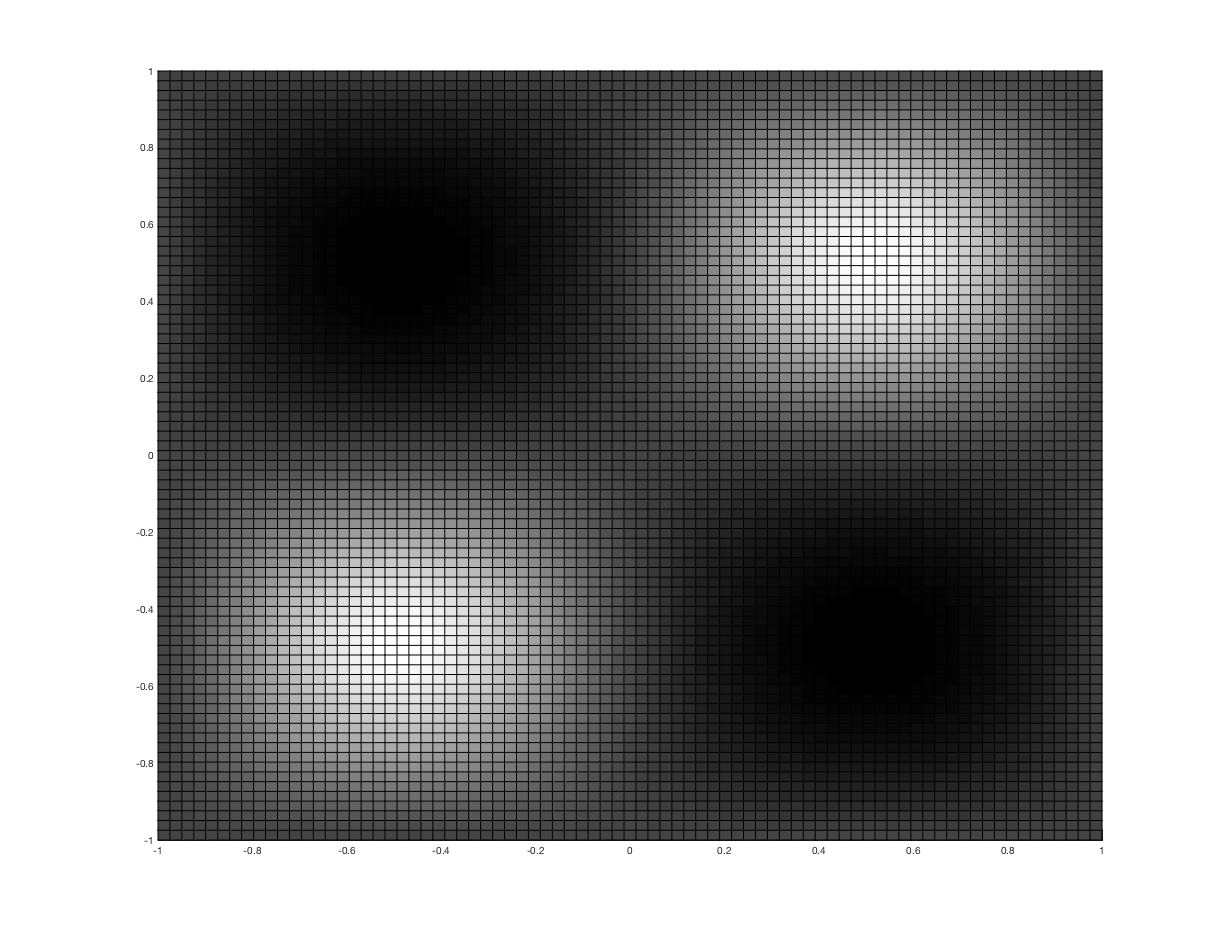
\includegraphics[scale=0.3]{Figures/02_03.png}
        \end{center}
        The following table shows the order of convergence, but I was unable to
        properly compute the energy error.
        \begin{center}
          \begin{tabular}{cccccc}
            \toprule
            M & h & Energy Error & Energy Order & L2 Error & L2 Order \\
            \midrule
             10 & 0.2    & - & - & 0.19      & -\\
             20 & 0.1    & - & - & 0.0357    & 2.283 \\
             40 & 0.05   & - & - & 0.007877  & 2.102 \\
             80 & 0.025  & - & - & 0.001867  & 2.039 \\
            %160 & 0.00625 & 0.013 & 2.05 & 0.0000004 & 0.065\\
            \bottomrule
          \end{tabular}
        \end{center}
    \end{enumerate}

  \item[\#2]
    Using the code posted online I was able to generate the following mesh for
    the given level set function.

    \begin{center}
      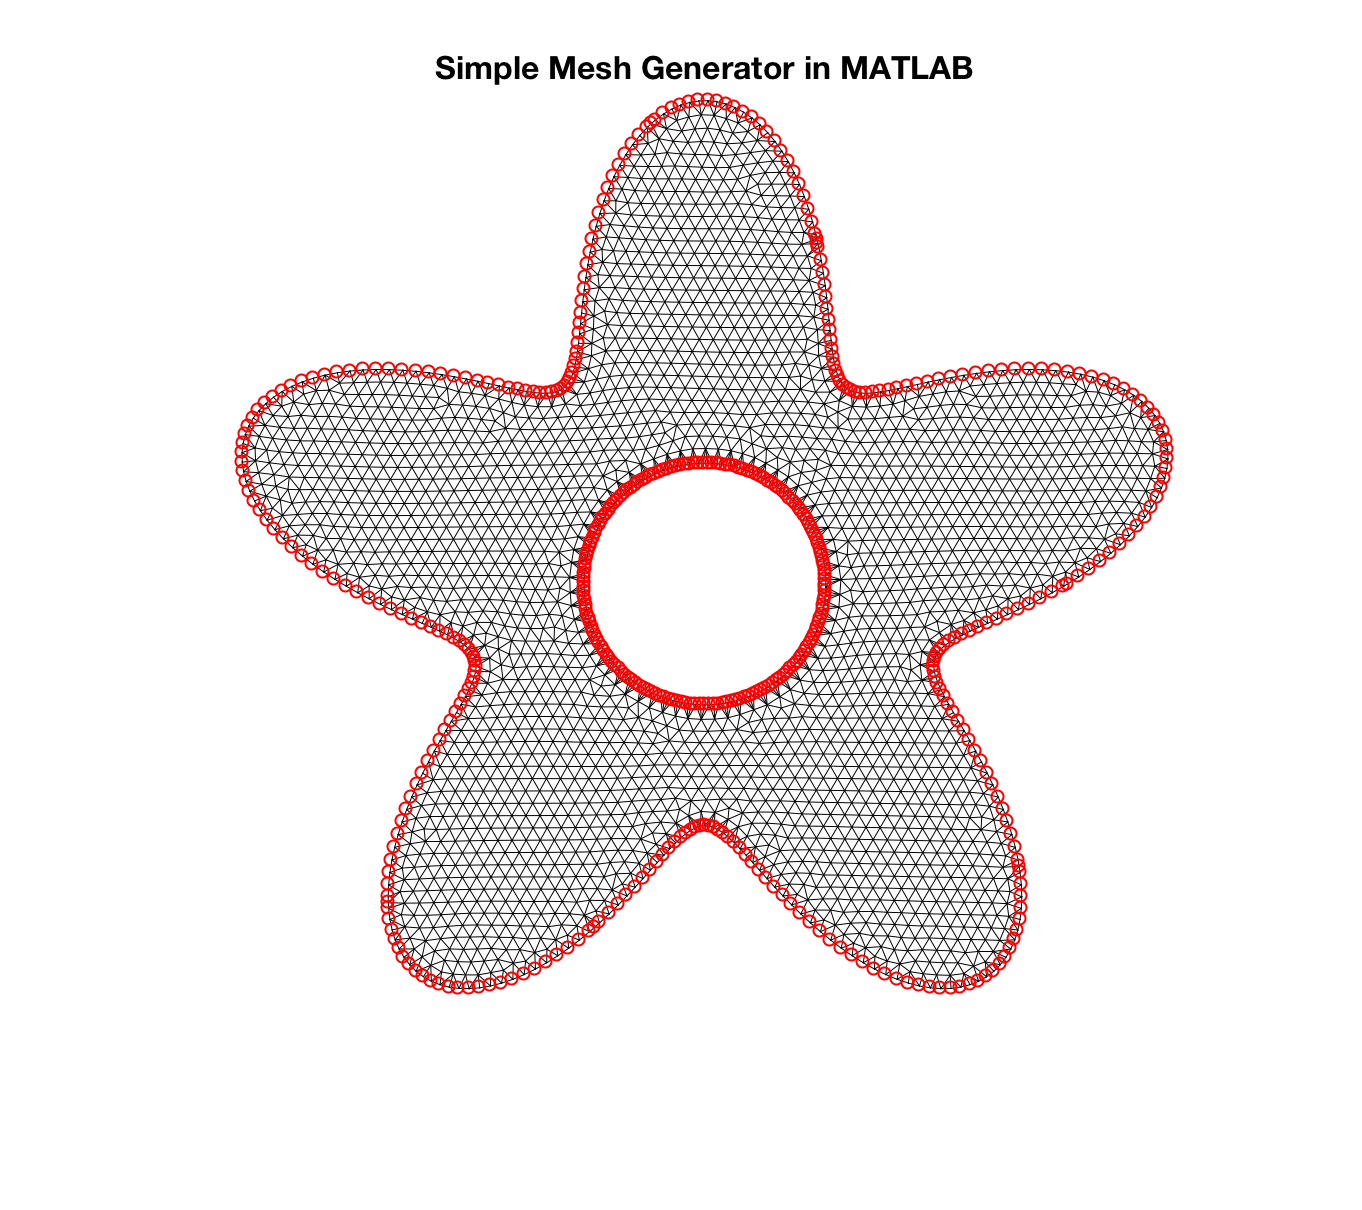
\includegraphics[scale=0.3]{Figures/02_01.png}
    \end{center}

  \item[\#3]
    The following code implements the cg1 method for any given triangulation in 2D.
    \lstinputlisting[language=MATLAB]{cg1_2D.m}

  \item[\#4]
    The following script uses the previous function to solve the poisson problem
    on the mesh found in problem 2.
    \lstinputlisting[language=MATLAB, firstline=49]{h02.m}

    \begin{center}
      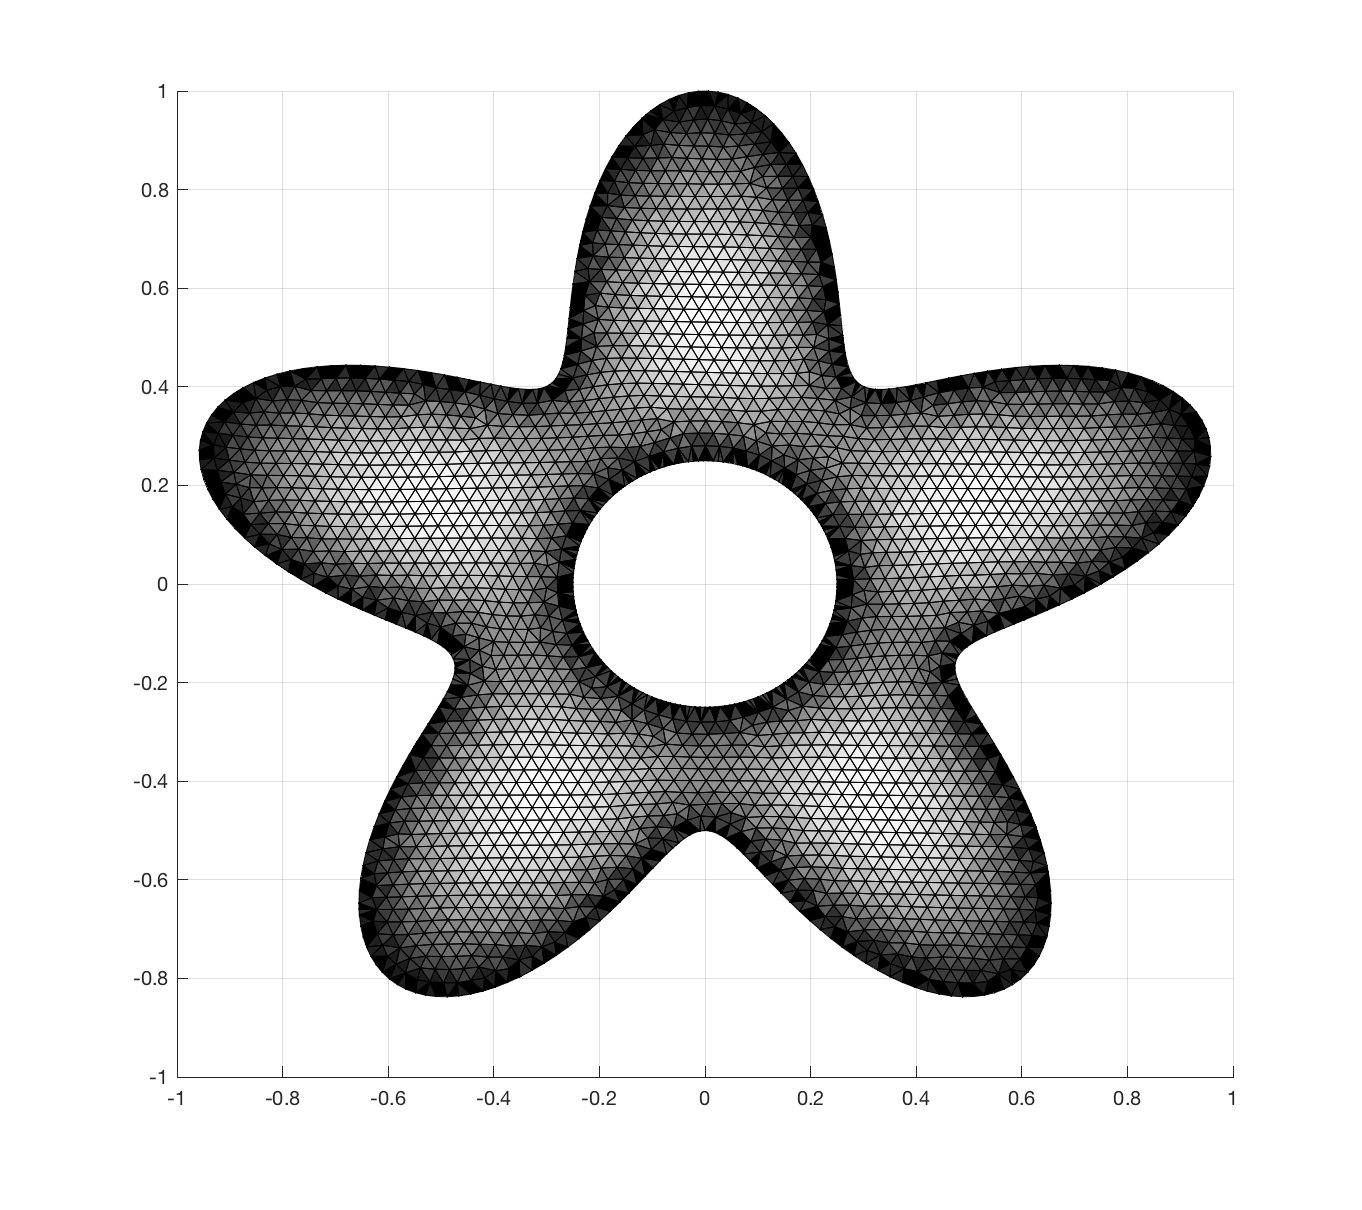
\includegraphics[scale=0.3]{Figures/02_02.png}
    \end{center}

\end{enumerate}
\end{document}
